%=======================02-713 LaTeX template, following the 15-210 template==================
%
% You don't need to use LaTeX or this template, but you must turn your homework in as
% a typeset PDF somehow.
%
% How to use:
%    1. Update your information in section "A" below
%    2. Write your answers in section "B" below. Precede answers for all 
%       parts of a question with the command "\question{n}{desc}" where n is
%       the question number and "desc" is a short, one-line description of 
%       the problem. There is no need to restate the problem.
%    3. If a question has multiple parts, precede the answer to part x with the
%       command "\part{x}".
%    4. If a problem asks you to design an algorithm, use the commands
%       \algorithm, \correctness, \runtime to precede your discussion of the 
%       description of the algorithm, its correctness, and its running time, respectively.
%    5. You can include graphics by using the command \includegraphics{FILENAME}
%
\documentclass[11pt]{article}
\usepackage{amsmath,amssymb,amsthm}
\usepackage{tikz}
\usetikzlibrary{arrows,positioning, calc}
\tikzstyle{vertex}=[draw,fill=black!15,circle,minimum size=20pt,inner sep=0pt]
\usepackage{graphicx}
\usepackage[margin=1in]{geometry}
\usepackage{fancyhdr}
\usepackage{mathtools}
\usepackage{placeins}
\usepackage{listings}
\usepackage{color}
\usepackage{forest}

\definecolor{dkgreen}{rgb}{0,0.6,0}
\definecolor{gray}{rgb}{0.5,0.5,0.5}
\definecolor{mauve}{rgb}{0.58,0,0.82}

\lstset{frame=none,
  language=Java,
  aboveskip=3mm,
  belowskip=3mm,
  showstringspaces=false,
  columns=flexible,
  basicstyle={\small\ttfamily},
  numbers=none,
  numberstyle=\tiny\color{gray},
  keywordstyle=\color{blue},
  commentstyle=\color{dkgreen},
  stringstyle=\color{mauve},
  breaklines=true,
  breakatwhitespace=true,
  tabsize=3
}

\setlength{\parindent}{0pt}
\setlength{\parskip}{5pt plus 1pt}
\setlength{\headheight}{13.6pt}
\newcommand\question[2]{\vspace{.25in}\hrule\textbf{#1 #2}\vspace{.5em}\hrule\vspace{.10in}}
\renewcommand\part[1]{\vspace{.10in}\textbf{(#1)}}
\newcommand\algorithm{\vspace{.10in}\textbf{Algorithm: }}
\newcommand\correctness{\vspace{.10in}\textbf{Correctness: }}
\newcommand\runtime{\vspace{.10in}\textbf{Running time: }}
\pagestyle{fancyplain}
\lhead{\textbf{\NAME}}
\chead{\textbf{HW\HWNUM}}
\rhead{\today}
\begin{document}\raggedright
%Section A==============Change the values below to match your information==================
\newcommand\NAME{Sean Connor (443-414-5111)}  % your name
\newcommand\HWNUM{ PA1}              % the homework number
%Section B==============Put your answers to the questions below here=======================

\question{Q1}{}
\part{a} First, let's look at binary search for this data structure. The recurrence relation for binary search is $T(n) = T(\frac{n}{2}) + O(1)$. We can apply the Master Theorem here, and see that $a=1$, $b=2$, and $f(n)=1$. This falls under Case 2, and so the complexity of binary search is O(lgn). We have two arrays - one of length $m$ and one of length $\sqrt{m}$. In the worst case, we would perform binary search on each, resulting in a time complexity of $O(lgm+lg\sqrt{m})$. This simplifies to $O(lgm + \frac{1}{2}lgm)$, or $O(\frac{3}{2}lgm)$. We see then that the overall time complexity is simply $O(lgn)$.

Determining the time complexity of inserting an element is trickier. In this, we insert into the small array until it is full, and then we merge the two arrays. Thus, merging occurs only occurs with every $\sqrt{m}$ insertions. The general time complexity of inserting into a sorted array is O(n); thus, inserting into the smaller array is $O(\sqrt{m})$ complexity. In addition, we know that merging two sorted arrays of size m and n is $O(m+n)$. In this case, merging would cost $O(m+\sqrt{m})$. This is the cost we need to cover using the the aggregate method described in the text. 

If we doubled the cost of each insertion to $2\sqrt{m}$, then between each merge we would have ``saved'' $\sqrt{m}\sqrt{m} = m$. However as seen above, merging costs more than this and so $2\sqrt{m}$ is not enough. If we instead charge $3\sqrt{m}$ per insertion, then between each merge we would have ``saved'' $2\sqrt{m}\sqrt{m} = 2m$. This covers the cost of the occasional merge. Since the total amortized cost is an upper bound on the total actual cost, and the amortized cost is $3\sqrt{m}$, we can say that the time complexity of insertion is $O(\sqrt{n})$.

\part{b} The code for this assignment can be found in the submitted .zip file, as well as in the appendix at the end of this document. This code has been slightly modified from what has been used for my own testing. The code provided will accept an input file by the user and present the sorted output. A brief description of my program follows. 

My program requires two arguments - an input filename/location and an output filename. The input files (provided) are .dat files containing an integer on each line. My program evaluates these input files and stores the integer values in an int[] array. The program iterates through the array of integers and used the insert() method to insert each one into the data structure described in the program document. Finally, the larger array of the data structure is output to the specified file.

To test, the program creates random integer arrays of varying lengths. Since we wanted to test time to insert the n\textsuperscript{th} item, the insert method is called n-1 times before using the system clock to time the final insert() method. I averaged insert() at n=10, 100, 1000, 10000, and 10000 over 1000 runs. Similarly, for binary search, I searched for a random index in array sizes of n=50, 500, 1000, 2000, 10000, and 20000 averaged over 1000 runs.

By inspection we can see that the primary methods involved here, sortedInsert() and merge(), perform at most $2\sqrt{m}$ and exactly $m+n$ calculations, respectively. To verify this, I utilized the system clock as I was unsure of any other method. As shown in Table 1 and Fig 1, the execution time for insert() has an upper bound of the expected $\sqrt{n}$. For binary search, the results were much more random and I was not able to verify execution time; however, the execution time across all values of n was very low ($<$ 2500 ns). See Table 2.


\begin{table}[!htbp]
\centering
\begin{tabular}{l|ll}
\textbf{n} & \textbf{Insert Time} \\ \hline
10                         & 475                  \\
100                        & 950                 \\
1000                      & 1524                 \\
10000                      & 4280                 \\
100000                     & 7103                               
\end{tabular}
\caption{Table of insert times (nanoseconds), averaged over 1000 runs for each value of n.}
\end{table}

\begin{table}[!htbp]
\centering
\begin{tabular}{l|ll}
\textbf{n} & \textbf{Search Time} \\ \hline
50                         & 886                  \\
500                        & 1904                 \\
1000                      & 2278                 \\
2000                      & 1901                 \\
5000                     & 1312                 \\
10000                    & 1379                 \\
20000                    & 1264                
\end{tabular}
\caption{Table of search times (nanoseconds), averaged over 1000 runs for each value of n.}
\end{table}

\begin{figure} [!htbp]
	\centering
	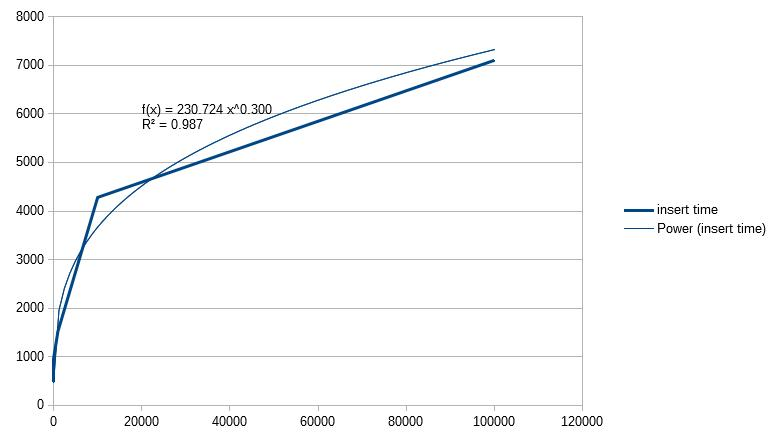
\includegraphics[width=6in]{graph1}
	\caption{Plot of time (nanoseconds) versus number of samples with a linear trendline. One thousand insertion tests were performed and average time was calculated at n=10, 100, 1000, 10000, and 100000.}
\end{figure}

\newpage

\section{Appendix}
\begin{lstlisting}
/**
 * This program is part of my response to PA 1 for the class 605.621
 * Foundations of Algorithms at the JHU EPP CS program.
 *
 * @author Sean Connor
 * @date 30 September 2018
 */

import java.io.*;
import java.util.*;
import java.time.LocalDateTime;

public class Main {

    public static void main(String[] args){

        // Create instance of Driver in order to use instance methods
        Main d = new Main();

        // Read filename from args if valid
        String[] input = d.readArgs(args);
        String filename = input[0];
        String output_filename = input[1];
        System.out.println("\nFilename: " + filename);

        // Extract data from input file
        int numLines = d.fileSize(filename);
        int[] data = d.readFile(filename,numLines);

        // Initialize random array for testing
        int[] ranArr = new int[1000];
        Random rand = new Random();

        // All data (large array, small array, and counter) is stored
        // in the 2D int[][] 'set'.
        // set[0] = counter
        // set[1] = large array
        // set[2] = small array
        int size = 1;
        int[][] set = new int[3][];
        set[0] = new int[1];
        set[1] = new int[size];
        set[2] = new int[(int)Math.floor(Math.sqrt(size))];

        long totalTime = 0;
        long startTime = 0;
        long endTime = 0;
        long deltaTime1 = 0;
        for (int i = 0; i < 1000; i++){
            // Generate random array of size n
            for (int j = 0; j < ranArr.length; j++){
                ranArr[j] = rand.nextInt(ranArr.length);
            }

            // Insert the first n-1 values
            for (int k = 0; k < ranArr.length-1; k++) {
                d.insert(ranArr[k],set);
            }

            // Calculate the time to insert the nth value
            startTime = System.nanoTime();
            d.insert(ranArr[ranArr.length-1],set); //
            endTime = System.nanoTime();
            deltaTime1 = endTime-startTime;
            totalTime = totalTime + deltaTime1;
        }
        long avgTime = totalTime/1000;
        System.out.println(avgTime);

        // Perform 1 binary search using random value between 0 and n.
        // Calculate time to complete.
        int rand_int;
        startTime = System.nanoTime();
        rand_int = rand.nextInt(data.length);
        int index = d.binarySearch(rand_int,set[1],set[2]);
        endTime = System.nanoTime();
        long deltaTime2 = endTime-startTime;

        // Write data to output file.
        StringBuilder output = d.arrayToFile(set[1], deltaTime1, deltaTime2, filename, rand_int, index);
        try (BufferedWriter bw = new BufferedWriter(new OutputStreamWriter(
                new FileOutputStream("../output/"+output_filename)))) {
            //new FileOutputStream(output_filename)))) {

            bw.write(output.toString());
        }
        catch (Exception e) {
            e.printStackTrace();
            System.out.println("\nFile not found. Please try again.\n");
            System.out.println();
            System.exit(1);
        }

    }


    /**
     * Method to ensure the proper number of arguments is given, and that the
     * filename given as an argument actually exists.
     *
     * @param args
     * @return   A string representing the filename to be read
     */
    private String[] readArgs(String[] args) {
        if (args.length == 2) {
            String filename = args[0];
            String output_filename = args[1];
            try {
                // Lazy file exists test
                File exists = new File(filename);
                Scanner exist_test = new Scanner(exists);
            } catch (FileNotFoundException exception) {
                System.out.println("\nFile not found.");
                System.exit(1);
            }
            String[] data = new String[2];
            data[0] = filename;
            data[1] = output_filename;
            return data;
        } else {
            System.out.println("\nInvalid number of arguments.");
            System.exit(1);
            return null;
        }
    }


    /**
     * Determines the number of lines in the input file. Returns in int
     * representing this value.
     *
     * @param filename
     * @return
     */
    private int fileSize(String filename) {

        try ( BufferedReader br = new BufferedReader(new InputStreamReader(
                new FileInputStream(filename))) ) {

            int counter = 0;
            String line;

            // Get number of lines in file
            while ( ( line = br.readLine() ) != null ) {
                // Check for empty line
                if ( line.equals("") ) {
                    System.out.println("\nError: Empty line found. Please check input.");
                    System.exit(1);
                }

                // Increment size counter
                counter++;
            }

            return counter;

        } catch (Exception e) {
            e.printStackTrace();
            System.out.println("\nFile not found. Please try again.\n");
            System.out.println();
            System.exit(1);
        }

        return 0;

    }


    /**
     * Runs through the file line by line and parses integer values to an
     * int[] array. Returns int[].
     *
     * @param filename
     * @param size
     * @return
     */
    private int[] readFile(String filename, int size) {
        try ( BufferedReader br = new BufferedReader(new InputStreamReader(
                new FileInputStream(filename))) ) {

            int counter = 0;
            String line;
            int[] data = new int[size];

            // Move through input file to parse int to array
            while ( ( line = br.readLine() ) != null ) {

                // Check for empty line
                if ( line.equals("") ) {
                    System.out.println("\nError: Empty line found. Please check input.");
                    System.exit(1);
                }

                // Parse int
                data[counter] = Integer.parseInt(line);

                // Increment counter to place in next array position
                counter++;
            }

            return data;

        } catch (Exception e) {
            e.printStackTrace();
            System.out.println("\nFile not found. Please try again.\n");
            System.out.println();
            System.exit(1);
        }

        return null;
    }


    /**
     * Create a string builder object with headers and relevant data appended.
     * Can be used by BufferedWriter to create output file.
     *
     * @param array
     * @param time
     * @return
     */
    private StringBuilder arrayToFile(int[] array, long time1, long time2, String filename, int term, int index) {

        StringBuilder output = new StringBuilder();
        output.append("Programming Assignment 1 - Output");
        output.append(System.getProperty("line.separator"));
        output.append("@author Sean Connor");
        output.append(System.getProperty("line.separator"));
        output.append("@date 1 October 2018");
        output.append(System.getProperty("line.separator"));
        output.append(System.getProperty("line.separator"));
        output.append("Filename: " + filename);
        output.append(System.getProperty("line.separator"));
        output.append("Calculation Date: " + LocalDateTime.now());
        output.append(System.getProperty("line.separator"));
        output.append("Insert Time (ns): " + time1);
        output.append(System.getProperty("line.separator"));
        output.append("Search Time (ns): " + time2);
        output.append(System.getProperty("line.separator"));
        output.append(System.getProperty("line.separator"));
        output.append("Searched for: " + term);
        output.append(System.getProperty("line.separator"));
        output.append("Found at index: " + index);
        output.append(System.getProperty("line.separator"));
        output.append(System.getProperty("line.separator"));

        for (int i = 0; i < array.length; i++) {

            output.append(array[i]);
            output.append(System.getProperty("line.separator"));

        }

        return output;

    }


    /**
     * This method inserts an integer value into a sorted integer array and
     * maintains the sorted status
     *
     * @param value
     * @param arr
     */
    private void sortedInsert(int value, int[] arr){
        for (int i = 0; i < arr.length; i++){
            if (value < arr[i]){
                for(int j = 1; j <= i; j++){
                    arr[j-1] = arr[j];
                }
                arr[i-1] = value;
                break;
            }

            else if (i == arr.length-1){
                for(int j = 1; j <= i; j++){
                    arr[j-1] = arr[j];
                }
                arr[i] = value;
            }
        }
    }


    /**
     * This method merges two sorted arrays into a third array of size m+n and
     * returns it.
     *
     * @param arr1
     * @param arr2
     * @return
     */
    private int[] mergeArrays(int[] arr1, int[] arr2){
        int[] result = new int[arr1.length+arr2.length];
        int i = 0;
        int j = 0;
        int k = 0;

        while (i < arr1.length && j < arr2.length){
            if (arr1[i] < arr2[j]){
                result[k] = arr1[i];
                i++;
                k++;
            }
            else {
                result[k] = arr2[j];
                j++;
                k++;
            }
        }

        while (i < arr1.length){
            result[k] = arr1[i];
            i++;
            k++;
        }

        while (j < arr2.length){
            result[k] = arr2[j];
            j++;
            k++;
        }

        return result;
    }


    /**
     * This is the primary insert method that utilizes sortedInsert() and
     * merge(). It relies on a counter to determine when to merge. When the
     * smaller array is filled, merge() will be called. The new larger array
     * will be the combined sorted array and the smalled array will be an empty
     * array with a size equal to the sqaure root of the larger array.
     *
     * @param value
     * @param set
     */
    private void insert(int value, int[][] set){
        // Insert value into small array and increment counter
        sortedInsert(value,set[2]);
        set[0][0]++;

        // If counter (set[0][0]) equals size of small array, small array is
        // full and need to merge arrays, reallocate, and reset counter.
        if (set[0][0] == set[2].length){
            set[0][0] = 0;
            set[1] = mergeArrays(set[1],set[2]);
            set[2] = new int[(int)Math.floor(Math.sqrt(set[1].length))];
        }
    }


    /**
     * This is a binary search method. It performs binary search on the larger
     * array first and the smaller array second. If the key is not found, the
     * method returns -1.
     *
     * @param value
     * @param data
     * @return
     */
    private int binarySearch(int value, int[] large, int[] small){
        // Check large array first
        int low = 0;
        int high = large.length-1;
        int mid;
        while (low <= high){
            mid = (int) Math.floor((low+high)/2);
            if (value < large[mid]){
                high = mid - 1;
            }
            else if (value > large[mid]){
                low = mid + 1;
            }
            else {
                return mid;
            }
        }

        // Check small array second
        low = 0;
        high = small.length-1;
        while (low <= high){
            mid = (int) Math.floor((low+high)/2);
            if (value < small[mid]){
                high = mid - 1;
            }
            else if (value > small[mid]){
                low = mid + 1;
            }
            else {
                return mid;
            }
        }

        // If not found, return -1
        return -1;
    }


}
\end{lstlisting}


\end{document}









